\documentclass[10pt,a4paper,twocolumn]{article}

\usepackage[T1]{fontenc}
\usepackage{lmodern}
\usepackage[a4paper,margin=0.69in,columnsep=0.23in]{geometry}
\usepackage{amsmath}
\usepackage{graphicx}
\usepackage{booktabs}
\usepackage{array}
\usepackage{caption}
\usepackage{xcolor}
\usepackage{float}
\usepackage[colorlinks=true,linkcolor=black,citecolor=blue,urlcolor=blue]{hyperref}
\usepackage{microtype}

\graphicspath{
  {../examples/demo_output/publication_figures/operating_v2/}
  {../examples/demo_output/publication_figures/s_bsst265/}
  {../examples/demo_output/operating_v2_eval/overlays/}
  {../examples/demo_output/s_bsst265_calibrated_eval/overlays/}
}

\captionsetup{font=small}
\setlength{\parindent}{0pt}
\setlength{\parskip}{1.2pt}
\setlength{\textfloatsep}{6pt plus 2pt minus 2pt}
\setlength{\floatsep}{5pt plus 2pt minus 2pt}
\setlength{\intextsep}{5pt plus 2pt minus 2pt}
\setlength{\emergencystretch}{1.5em}
\renewcommand{\arraystretch}{1.10}
\raggedbottom
\newcolumntype{L}[1]{>{\raggedright\arraybackslash}p{#1}}

\begin{document}

\twocolumn[
\begin{center}
{\LARGE\bfseries ClusterCount-AI4S:\par}
\vspace{4pt}
{\LARGE\bfseries robust cell-count validation under clustering, blur, and domain shift\par}
\vspace{12pt}
{\large Thato Baruti\par}
\vspace{2pt}
{\textit{Independent study}\par}
\vspace{8pt}
18 May 2026\par
\end{center}

\begin{abstract}
Automated cell counting in fluorescence microscopy is not only a segmentation problem; it is a measurement-validity problem. When nuclei cluster, blur erodes boundaries, and acquisition conditions shift across laboratories, magnifications, or sample preparations, a visually plausible output can still yield an unreliable count. This report evaluates ClusterCount-AI4S as a validation framework built around two complementary model classes: \textbf{ClusterCountModel}, an interpretable regressor used for controlled operating-range benchmarking, and a calibrated patchwise density pipeline used for direct external adaptation. Controlled experiments on 300 held-out synthetic test images show 4.67\% mean absolute percentage error, improving to 4.45\% within a moderate blur and clustering envelope. External evaluation on a heterogeneous microscopy benchmark derived from the BioStudies accession S-BSST265 shows that scale-normalized patchwise inference followed by lightweight calibration reduces held-out external MAPE to 34.3\%, improving on the raw patchwise model while still leaving substantial failure in high-count and cross-regime scenes. Rather than treating these limits as an inconvenience, the framework makes them central to interpretation through explicit warnings, model-baseline disagreement, and image-level overlays. The study therefore contributes a reproducible validation protocol for count reliability, not a claim of universal superiority over established segmentation systems.
\end{abstract}

\noindent\textbf{Key words:} Biomedical image analysis -- Fluorescence microscopy -- Cell counting -- Domain shift -- Uncertainty -- Validation
\vspace{0.45cm}
]

\section{Framing the problem}

\subsection{Why counting reliability deserves its own benchmark}
Cell counting is often discussed through the lens of instance segmentation, yet the scientific quantity of interest is frequently the aggregate number of valid nuclei or cells per field of view. Those two objectives overlap but are not identical. In dense preparations, two models can produce qualitatively different boundaries while agreeing on count, and conversely, a visually reasonable segmentation may still undercount merged nuclei or overcount texture fragments. This is particularly relevant in fluorescence microscopy, where blur, variable signal-to-noise ratio, and clustered nuclei produce ambiguity at exactly the point where biological conclusions become count-sensitive.

Established systems such as Cellpose, StarDist, and CellProfiler have already demonstrated the value of robust segmentation and analysis pipelines across many image types \cite{cellpose,stardist,cellprofiler}. The question addressed here is therefore narrower and more operational: \emph{under what conditions can an automated count be trusted, and what evidence should accompany that count when it should not?}

\subsection{Position of the present study}
ClusterCount-AI4S addresses that question by separating \emph{model development} from \emph{count validation}. The repository contains both a tiny density-map CNN prototype, reflecting the density-integration view of object counting \cite{lempitsky}, and \textbf{ClusterCountModel}, an interpretable count regressor trained on synthetic microscopy descriptors. The present report uses those model classes differently. ClusterCountModel remains the principal operating-range model because it retrains quickly, converges stably, and makes feature-driven failure modes easy to audit. For the external benchmark, the best current path is a directly supervised patchwise density CNN with magnification-aware resizing, patchwise intensity standardization, output-scale initialization, and relative-count losses, followed by a lightweight calibration stage that uses watershed disagreement and count dispersion as corrective signals.

\section{Data foundation and evaluation protocol}

\subsection{Synthetic data as a controlled perturbation space}
The synthetic benchmark was designed to isolate two failure drivers that recur in practice: optical blur and spatial clustering. It contains 3000 fluorescence-like microscopy images split into 2400 training, 300 validation, and 300 test images. Because object counts are exact by construction, synthetic data provide a clean environment for measuring systematic count error without annotation disagreement. They are particularly useful when the aim is not to claim biological realism in every detail, but to stress-test whether a model preserves count under controlled degradations.

\subsection{External benchmark from S-BSST265}
The external dataset source is the BioStudies fluorescence microscopy study \texttt{S-BSST265} (\href{https://www.ebi.ac.uk/biostudies/bioimages/studies/S-BSST265}{BioStudies study page}), released with detailed annotations by Kromp et al. \cite{kromp_dataset,kromp_biostudies}. The full resource contains 79 images and 7813 nuclei across multiple diagnoses, preparations, modalities, magnifications, and signal-to-noise regimes \cite{kromp_dataset}. In the current repository, a 37-image held-out slice is used as an external stress test rather than an in-distribution validation set.

This provenance matters. The S-BSST265 annotation protocol explicitly restricts labels to intact, in-focus nuclei and excludes heavily distorted or ambiguous structures \cite{kromp_dataset}. Count performance must therefore be interpreted relative to a biologically informed annotation policy rather than an unconstrained notion of ``all visible objects.'' That is a strength, not a weakness: it aligns the benchmark with the reality that microscopy counts are always conditioned on annotation criteria.

\begin{table}[H]
\centering
\footnotesize
\begin{tabular}{L{0.26\linewidth} L{0.29\linewidth} r}
\toprule
\textbf{Benchmark} & \textbf{Role in study} & \textbf{Images} \\
\midrule
Synthetic training split & Fit ClusterCountModel & 2400 \\
Synthetic validation split & Capacity selection and convergence & 300 \\
Synthetic test split & Controlled operating-range benchmark & 300 \\
S-BSST265 test slice & External domain-shift stress test & 37 \\
\bottomrule
\end{tabular}
\caption{Evaluation partitions used in the present report.}
\label{tab:splits}
\end{table}

\subsection{Relation to public benchmark resources}
Although the results below focus on synthetic data and S-BSST265, the study is aligned with the broader benchmarking culture represented by the Broad Bioimage Benchmark Collection and by cross-experiment nuclei datasets such as the 2018 Data Science Bowl resource \cite{ljosa,bbbc004,bbbc005,dsb2018}. These benchmarks are important because they encourage methodological claims to be grounded in reproducible stress tests rather than single-dataset success cases.

\section{ClusterCountModel and baseline methodology}

\subsection{Model definition}
For an input image $x$, ClusterCountModel predicts a count
\begin{equation}
\hat{c}=f_{\theta}(\phi(x)),
\end{equation}
where $\phi(x)$ is a feature vector derived from interpretable image statistics: global intensity mass, thresholded foreground occupancy, high-percentile brightness, gradient magnitude, Laplacian sharpness, smoothed intensity totals, and peak-count proxies. The regressor itself is an ensemble of extremely randomized trees \cite{extratrees}, chosen because this family is fast, stable on modest sample sizes, and naturally exposes tree-wise variation that can be recycled into an uncertainty heuristic.

For external adaptation, the repository also includes a patchwise density CNN. Large images are first rescaled toward a reference magnification, decomposed into overlapping patches, standardized patchwise, and mapped to density targets whose integrals equal local nucleus counts. Naive density regression was not sufficient on its own: without output-bias initialization and relative-count terms in the loss, the network could converge toward near-zero densities on externally shifted data. The selected external configuration therefore adds a post-hoc calibrator that combines the raw patchwise count, the watershed count, the patchwise uncertainty estimate, and model-baseline disagreement in a compact ensemble regressor. This is not framed as a universal fix; it is a pragmatic method-selection result grounded in the observed external benchmark.

\subsection{Why an interpretable regressor rather than end-to-end segmentation}
Counting under overlap can be approached by instance segmentation, density integration, or direct regression. Density-based formulations are attractive because they decouple count from exact contour delineation \cite{lempitsky}. In the current repository, the fully validated operating-range model is nonetheless a tabular-image hybrid: rich image descriptors plus a tree ensemble. This configuration is pragmatic rather than doctrinal. It allows rapid retraining, explicit convergence analysis, feature-importance inspection, and straightforward comparison with a classical baseline, which are all useful properties in a benchmark report. The patchwise CNN is then used not to replace that benchmark logic, but to test how far direct supervision can reduce external-count error when the domain-shift problem is tackled more locally.

\subsection{Baseline and confidence heuristic}
The principal baseline is a watershed count extractor \cite{watershed}. Watershed is not merely a comparator; it also supplies a disagreement signal at inference time. If $\sigma_{\text{model}}$ denotes model-specific count dispersion, $d_{\text{ws}}$ the normalized disagreement between the learned model and watershed, and $b(x)$ the blur estimate, the deployed confidence score follows the form
\begin{equation}
\mathrm{conf}(x)\approx 1-\left(0.35\frac{\sigma_{\text{model}}}{\max(\hat{c},1)}+0.35d_{\text{ws}}+0.30b(x)\right),
\end{equation}
clipped to the unit interval. In the tree model, $\sigma_{\text{model}}$ is estimated from ensemble variation; in the CNN path it can be approximated by repeated stochastic forward passes. This score is heuristic rather than probabilistically calibrated, but it reflects an important principle from the uncertainty literature: trust should not be inferred from point predictions alone, especially under dataset shift \cite{ovadia}.

\section{Results}

\subsection{Controlled operating-range behavior}
ClusterCountModel converged smoothly as the number of trees increased from 50 to 1000. Validation MAPE decreased from 5.27\% at 50 trees to 5.11\% at 1000 trees, with diminishing returns after roughly 400 trees. This shape argues against a fragile optimum and suggests that the model is operating in a relatively stable capacity regime.

\begin{figure}[H]
\centering

\includegraphics[width=\linewidth]{convergence.png}
\caption{ClusterCountModel convergence across the tree schedule. The dashed line marks the 5\% MAPE target.}
\label{fig:convergence}
\end{figure}

On the held-out synthetic test split, ClusterCountModel achieved \textbf{4.67\% MAPE}, \textbf{1.39 MAE}, and \textbf{1.81 RMSE} across 300 images, whereas watershed reached \textbf{31.71\% MAPE}, \textbf{11.03 MAE}, and \textbf{13.20 RMSE}. Within the stricter operating envelope defined by \texttt{blur\_sigma $\leq$ 0.9} and \texttt{cluster\_strength $\leq$ 0.30}, error tightened further to \textbf{4.45\% MAPE} across 63 images.

The regime summary is informative. Across the tested synthetic split, the blur buckets remained almost flat in relative error (about 4.6--4.7\%), whereas the clustering buckets separated more clearly: MAPE rose from 4.26\% in the lower-clustering subset to 5.07\% in the medium-clustering subset. In other words, within this benchmark, clustering perturbs the count more strongly than blur once blur remains inside the modeled operating envelope.

\begin{table}[H]
\centering
\footnotesize
\begin{tabular}{L{0.29\linewidth} c c}
\toprule
\textbf{Metric} & \textbf{ClusterCountModel} & \textbf{Watershed} \\
\midrule
Held-out images & 300 & 300 \\
MAE & 1.39 & 11.03 \\
RMSE & 1.81 & 13.20 \\
MAPE & \textbf{4.67\%} & 31.71\% \\
Median absolute error & 1.09 & 10.00 \\
Maximum absolute error & 5.75 & 33.00 \\
\bottomrule
\end{tabular}
\caption{Controlled synthetic benchmark results.}
\label{tab:synthetic}
\end{table}

\subsection{Auditability in success and failure regimes}
The synthetic overlay confirms the intended operating behavior: under moderate blur and limited clustering, detected peaks align with visible nuclei and the count remains numerically close to ground truth. The external overlay tells a different story. On \texttt{otherspecimen\_6}, the true count is 969 whereas the calibrated external model predicts 323.9 and watershed predicts 1024. The value of the framework is that this residual failure does not remain hidden inside an aggregate metric. It is visible in the image, surfaced in the warning string, and reinforced by disagreement with the watershed baseline.

\begin{figure}[H]
\centering
\begin{minipage}[t]{0.48\linewidth}
\centering
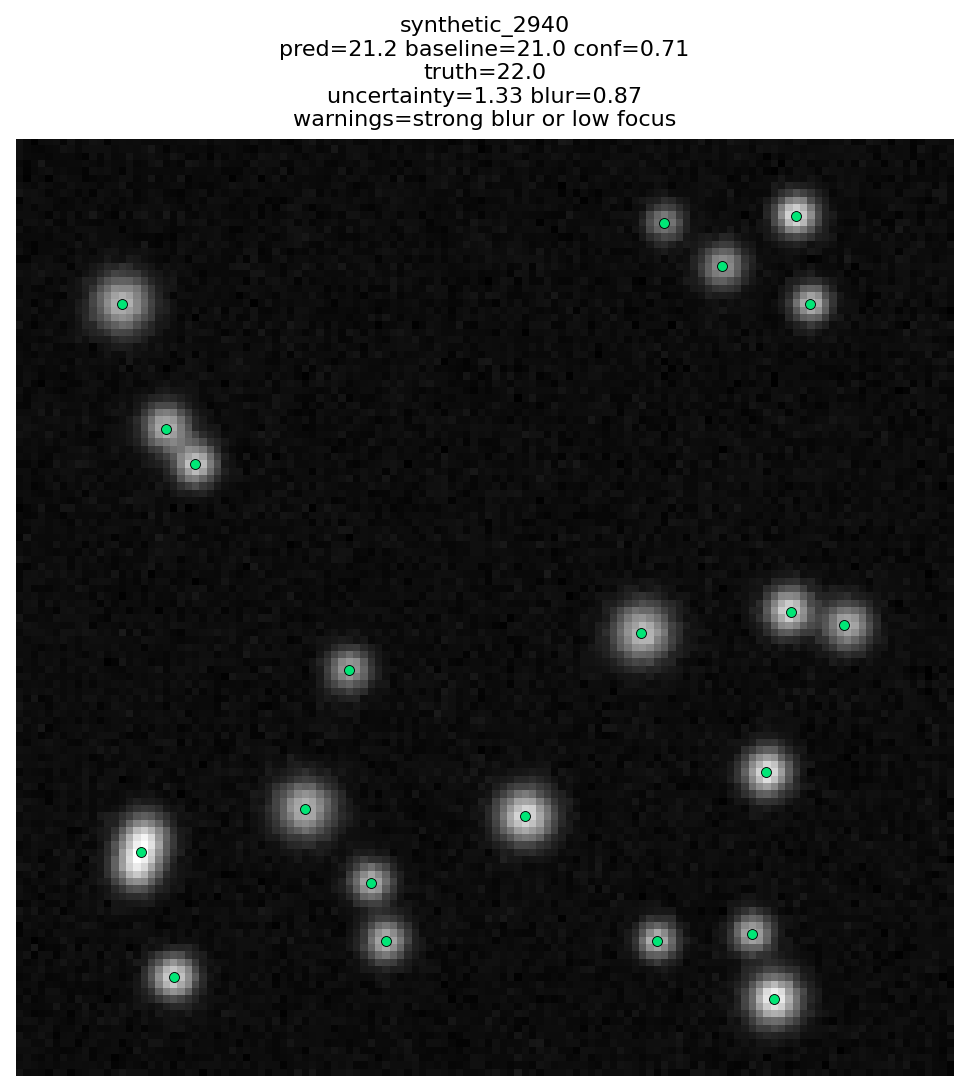
\includegraphics[width=\linewidth]{synthetic_2940_overlay.png}
\end{minipage}
\hfill
\begin{minipage}[t]{0.48\linewidth}
\centering
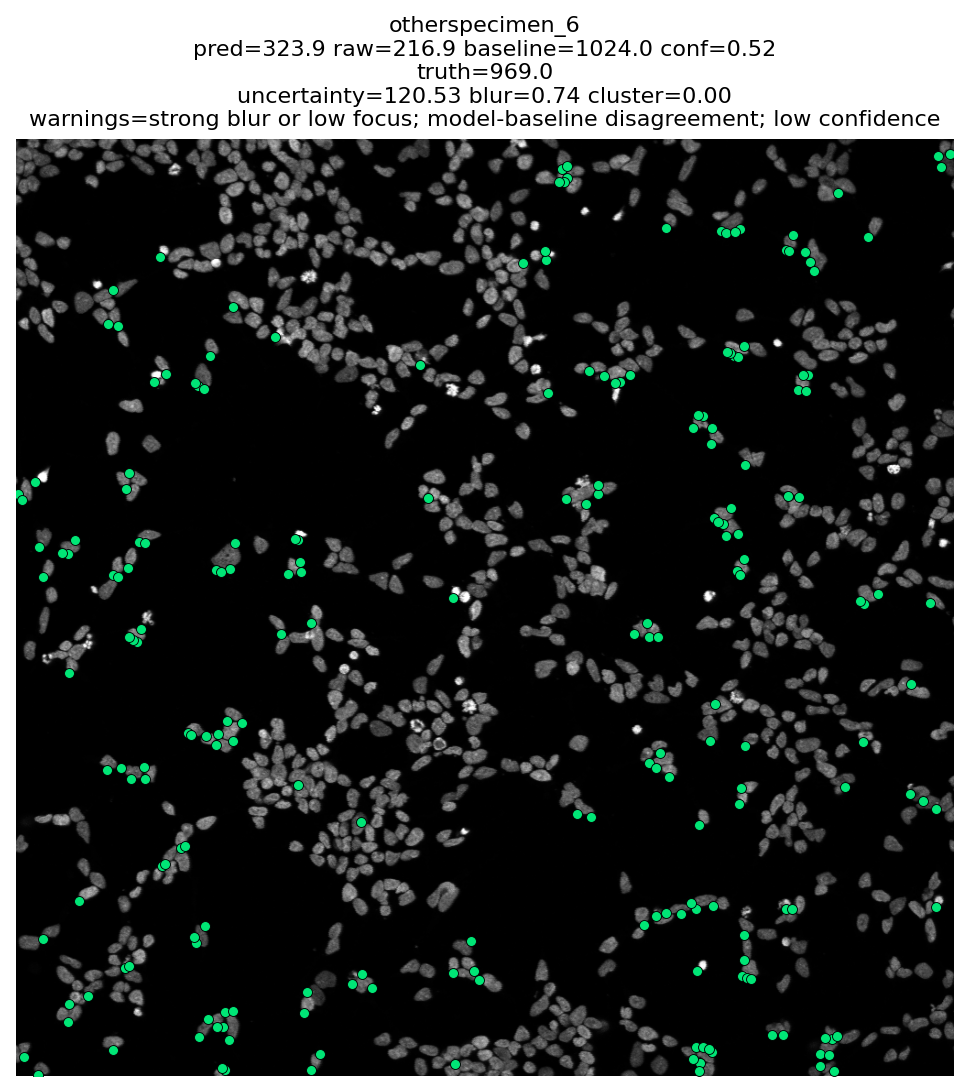
\includegraphics[width=\linewidth]{otherspecimen_6_overlay.png}
\end{minipage}
\caption{Image-level auditability. Left: representative synthetic success case with true count 22 and predicted count 21.2. Right: external failure case from S-BSST265 with true count 969 and predicted count 323.9 after calibration-aware external adaptation.}
\label{fig:overlays}
\end{figure}

\subsection{External behavior under domain shift}
The external benchmark is the most important result in the report because it limits the scope of what can be claimed. Among the implemented external paths, the best current configuration is the calibrated patchwise model. On the 37-image S-BSST265 slice, it achieved \textbf{34.3\% MAPE}, improving on the raw scale-normalized patchwise CNN at \textbf{36.5\% MAPE} and substantially outperforming watershed on proportional error (\textbf{134.85\% MAPE}). The calibrated model also reduced median absolute error from 18.8 to 12.6 cells. This shows that local patchwise reasoning, magnification-aware normalization, and light post-hoc calibration improve proportional accuracy under domain shift.

At the same time, the result remains far from deployment-safe. Even after calibration, the maximum absolute error still reached 645.10 cells, and the error profile is strongly regime-dependent. Watershed retained lower RMSE because it stayed closer on some ultra-dense fields, whereas its MAPE was much worse because it over-segmented several low-count images. Different metrics therefore reward different operating behaviors, and no single scalar should be used to declare the external problem solved. The same evidence explains why the center-heatmap U-Net was not selected: on the current heterogeneous split, it was materially less stable than the calibrated patchwise alternative.

The remaining failures are consistent with the structure of the source dataset. Kromp et al. explicitly describe heterogeneity across diagnosis, preparation type, magnification, modality, and signal-to-noise ratio \cite{kromp_dataset}. In the present evaluation, the hardest residual errors concentrated in high-count 20x scenes, LSM images, and the \texttt{otherspecimen\_*} subset. The benchmark is therefore useful not only for reporting a single external number, but for identifying which regimes would require a stronger center-point or instance-level model before sub-5\% performance could be considered realistic.

\begin{table}[H]
\centering
\scriptsize
\begin{tabular}{L{0.20\linewidth} c c c}
\toprule
\textbf{Metric} & \textbf{Calibrated} & \textbf{Raw} & \textbf{Watershed} \\
\midrule
Held-out images & 37 & 37 & 37 \\
MAE & \textbf{55.61} & 66.47 & 60.35 \\
RMSE & 138.71 & 148.13 & \textbf{85.41} \\
MAPE & \textbf{34.33\%} & 36.54\% & 134.85\% \\
Median abs. error & \textbf{12.61} & 18.80 & 40.00 \\
Max abs. error & 645.10 & 752.15 & \textbf{233.00} \\
\bottomrule
\end{tabular}
\caption{External S-BSST265 stress-test results. The calibrated patchwise model is the best current learned configuration on proportional error and median absolute error.}
\label{tab:external}
\end{table}

\section{Interpretation}
Two conclusions follow directly from the evidence. First, ClusterCountModel is a competent counter within a defined operating range. The synthetic benchmark shows that when blur and clustering remain close to the modeled conditions, count error can be kept below 5\% without requiring full instance segmentation. Second, external performance is highly architecture- and regime-dependent. A dedicated patchwise density CNN trained directly on S-BSST265 reduces proportional external error substantially, and a lightweight calibration layer improves it further, but morphology, acquisition, and preparation shift still dominate performance in the hardest scenes.

That asymmetry is scientifically useful. A validation-first tool should make its failure surface explicit so that downstream users can decide when a count is adequate for exploratory quantification, when review is required, and when task-specific adaptation is unavoidable. In the present case, the evidence suggests that sub-5\% external MAPE would require a different class of model again: likely a center-point or instance-level detector, trained directly on the external masks and stratified by acquisition regime. The calibrated patchwise route is therefore best interpreted as the \emph{current best external compromise}, not as the endpoint of the method. In that sense, the present framework is better understood as an \emph{auditable reliability study} than as a universal counting solution.

\section{Key takeaways}
\begin{itemize}
\item ClusterCountModel is the principal validated model in the repository; it is an interpretable extremely randomized trees regressor built on microscopy-derived descriptors.
\item Controlled synthetic evaluation reaches 4.67\% MAPE on 300 held-out images and 4.45\% MAPE inside a moderate blur and clustering envelope.
\item Within the evaluated synthetic range, clustering perturbs counts more strongly than blur.
\item The best current external method is a calibrated patchwise density pipeline, which improves S-BSST265 test MAPE to 34.3\% and median absolute error to 12.6 while still remaining well above a deployment-safe threshold.
\item The raw patchwise model and watershed baseline remain scientifically useful because they show, respectively, the value of local density reasoning and the metric trade-off between proportional and absolute error in ultra-dense scenes.
\item The most valuable output of the framework is not only the count, but the accompanying evidence: overlays, disagreement signals, blur-sensitive warnings, and explicit operating-range limits.
\end{itemize}

\section{References}
\scriptsize
\begin{thebibliography}{13}
\setlength{\itemsep}{0.2ex}
\setlength{\parskip}{0pt}

\bibitem{kromp_dataset}
Kromp F, Bozsaky E, Rifatbegovic F, et al.
\newblock An annotated fluorescence image dataset for training nuclear segmentation methods.
\newblock \emph{Scientific Data} 7, 262 (2020).
\newblock \href{https://doi.org/10.1038/s41597-020-00608-w}{doi:10.1038/s41597-020-00608-w}

\bibitem{kromp_biostudies}
Kromp F, Bozsaky E, Rifatbegovic F, et al.
\newblock BioStudies accession S-BSST265: annotated fluorescence image dataset for training nuclear segmentation methods (2020).
\newblock \url{https://www.ebi.ac.uk/biostudies/bioimages/studies/S-BSST265}

\bibitem{cellpose}
Stringer C, Wang T, Michaelos M, Pachitariu M.
\newblock Cellpose: a generalist algorithm for cellular segmentation.
\newblock \emph{Nature Methods} 18, 100--106 (2021).
\newblock \href{https://doi.org/10.1038/s41592-020-01018-x}{doi:10.1038/s41592-020-01018-x}

\bibitem{stardist}
Schmidt U, Weigert M, Broaddus C, Myers G.
\newblock Cell Detection with Star-convex Polygons.
\newblock In \emph{Medical Image Computing and Computer Assisted Intervention} (MICCAI), 2018.
\newblock \href{https://arxiv.org/abs/1806.03535}{arXiv:1806.03535}

\bibitem{cellprofiler}
McQuin C, Goodman A, Chernyshev V, et al.
\newblock CellProfiler 3.0: next-generation image processing for biology.
\newblock \emph{PLOS Biology} 16(7), e2005970 (2018).
\newblock \href{https://doi.org/10.1371/journal.pbio.2005970}{doi:10.1371/journal.pbio.2005970}

\bibitem{dsb2018}
Caicedo JC, Goodman A, Karhohs KW, et al.
\newblock Nucleus segmentation across imaging experiments: the 2018 Data Science Bowl.
\newblock \emph{Nature Methods} 16, 1247--1253 (2019).
\newblock \href{https://doi.org/10.1038/s41592-019-0612-7}{doi:10.1038/s41592-019-0612-7}

\bibitem{ljosa}
Ljosa V, Sokolnicki KL, Carpenter AE.
\newblock Annotated high-throughput microscopy image sets for validation.
\newblock \emph{Nature Methods} 9, 637 (2012).
\newblock \href{https://doi.org/10.1038/nmeth.2083}{doi:10.1038/nmeth.2083}

\bibitem{bbbc004}
Broad Bioimage Benchmark Collection.
\newblock BBBC004: synthetic fluorescent cell images for overlap stress testing.
\newblock \url{https://bbbc.broadinstitute.org/BBBC004/}

\bibitem{bbbc005}
Broad Bioimage Benchmark Collection.
\newblock BBBC005: synthetic fluorescent cell images with controlled count and blur variation.
\newblock \url{https://bbbc.broadinstitute.org/BBBC005/}

\bibitem{lempitsky}
Lempitsky V, Zisserman A.
\newblock Learning to count objects in images.
\newblock In \emph{Advances in Neural Information Processing Systems} 23, 2010.
\newblock \href{https://papers.nips.cc/paper/2010/hash/fe73f687e5bc5280214e0486b273a5f9-Abstract.html}{NeurIPS 2010}

\bibitem{extratrees}
Geurts P, Ernst D, Wehenkel L.
\newblock Extremely randomized trees.
\newblock \emph{Machine Learning} 63, 3--42 (2006).
\newblock \href{https://services.montefiore.uliege.be/stochastic/pubs/2006/GEW06a/}{publisher page}

\bibitem{watershed}
Vincent L, Soille P.
\newblock Watersheds in digital spaces: an efficient algorithm based on immersion simulations.
\newblock \emph{IEEE Transactions on Pattern Analysis and Machine Intelligence} 13(6), 583--598 (1991).

\bibitem{ovadia}
Ovadia Y, Fertig E, Ren J, et al.
\newblock Can you trust your model's uncertainty? Evaluating predictive uncertainty under dataset shift.
\newblock In \emph{Advances in Neural Information Processing Systems} 32, 2019.
\newblock \href{https://papers.nips.cc/paper/9547-can-you-trust-your-models-uncertainty-evaluating-predictive-uncertainty-under-dataset-shift}{NeurIPS 2019}

\end{thebibliography}

\vspace{6pt}
\textit{Disclaimer: Independent, non-clinical methodological study. ClusterCount-AI4S is presented as a validation framework for robust cell counting under clustering, blur, and domain shift rather than as a universally solved counting system.}

\end{document}
